\documentclass{article}
\usepackage{graphicx} % Required for inserting images

\title{2048}
\author{Christina Liu}
\date{November 2023}

%% \blurb{help}

\begin{document}

\maketitle

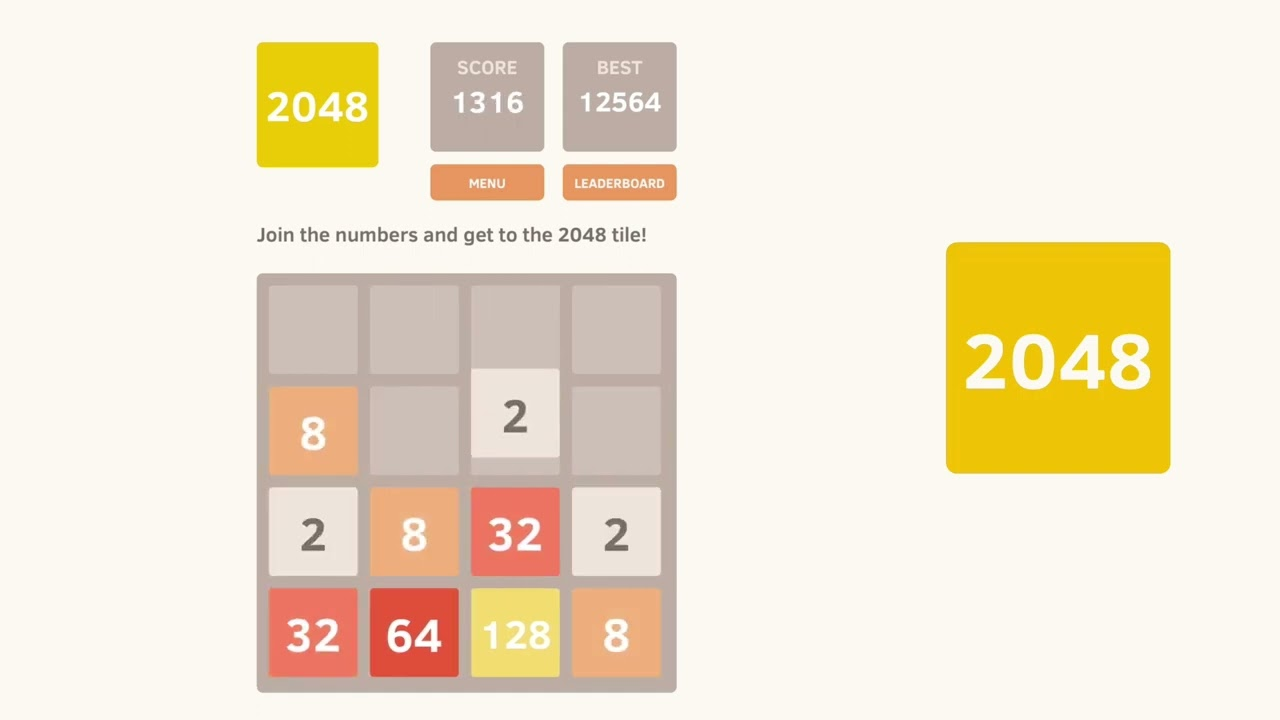
\includegraphics[height=3in]{images/2048_preview.png}

I’m pretty sure literally everyone on the planet has played this game before. 2048 is a classic. Even with its minimalistic setup and nerdy block-sliding gameplay, you can’t doubt that it’s iconic. It’s easy to understand, yet hard to master, the perfect recipe for a kind of brain-rotting gaming rage that keeps you coming back through sheer frustration. And as a bonus, you get to quickly and naturally remember powers of two as you attempt to reach new numbers. Truly, 2048 was a viral hit.

But despite its seemingly effortless success, there are some unseen bits of history behind this beloved slice of our childhoods that aren’t really talked about. Turns out, this little game with a beige background and warm multicolored tiles has a quite interesting past.
\newline

2048’s inspiration came from a game called Threes!. Developers Asher Vollmer, Greg Wohlwend, and Jimmy Hinson created a hit \$2 mobile game that required you to combine tiles using the same sliding block mechanics as 2048, but with a little twist. For numbers 3 and above, the same matching mechanics apply, but when 1 and 2 tiles pop up, they must be combined to make 3. This game was quite popular, with many articles written dedicated to strategies to beat it. At one point, it was even on the top of the paid chart in the App store. In Threes, most of 2048’s core mechanics had already been set in stone. Someone just needed to come along and make a few minor tweaks.

1024! was dropped on the iOS app store by Veewo Studios just around a month after the success of Threes!. This new game kept the framework the same while replacing the multiples of 3s with powers of 2. Gameplay seems to be similar to that of 2048, except for a static 0 block that hinders the sliding movement of some turns. This game also enjoyed a nice bit of success, especially considering its rise from the many clones of Threes!. Seeing the success of both Threes! and 1024!, even more derivative games began popping up everywhere.

Among the clones of 1024!, one stood out: 2048 by then 19-year-old developer Gabriele Cirulli. 2048 took all of the mechanics of 1024!, removed the 0 block, and sped up the animations to create a clean, fast, minimalistic, and addictive experience. From here, the game blew up. Cirulli released the game on Github, where players racked up more than 33 million plays in just one week. But with such a complex past, it’s difficult to decide who to attribute the success of 2048 to.

Truly, the success of 2048 wasn’t just a one-step success. Even with seemingly simple game mechanics, the game had to be passed through the hands of several developers to reach its viral success. Maybe one day, we’ll see the arrival of 4096, an even faster paced math game that will once again dominate the charts.

Sidenote: (Perhaps continuing in the spirit of 2048’s creation, it’s interesting to note that the iPhone version of 2048 that many people use to play is not distributed by Cirulli.)
\end{document}https://www.overleaf.com/project/64fdffc729fe724646250530